% =============================================================
%  FRONTESPIZIO TEMPLATE  –  stile "Technical Research Report"
%  Basato sul layout del documento FDA-CP (Duyar, 2026)
%  Adattato per report tecnici Leitner / PCIM / DAB / LeitDrive
% =============================================================
\documentclass[12pt, a4paper]{article}

% ---- Pacchetti base ----
\usepackage[T1]{fontenc}
\usepackage[utf8]{inputenc}
\usepackage[english]{babel}          % cambia in [italian] se serve
\usepackage{geometry}
\usepackage{xcolor}
\usepackage{tikz}
\usepackage{graphicx}
\usepackage{amsmath}
\usepackage{amssymb}


\usepackage{hyperref}
\usepackage{booktabs}
\usepackage{array}
\usepackage{tabularx}
\usepackage{mdframed}                % box abstract

% ---- Margini pagina ----
\geometry{
    a4paper,
    top    = 2.5cm,
    bottom = 2.5cm,
    left   = 2.8cm,
    right  = 2.8cm
}

% ---- Colori (palette del report originale) ----
\definecolor{headerblue}{RGB}{40, 80, 140}     % blu titolo principale
\definecolor{subtlegray}{RGB}{100, 100, 100}   % grigio per metadati
\definecolor{ruleblue}{RGB}{60, 110, 180}      % linea decorativa
\definecolor{boxbg}{RGB}{245, 247, 252}        % sfondo box author/date
\definecolor{abstractbg}{RGB}{240, 244, 250}   % sfondo box abstract

% ---- Hyperref setup ----
\hypersetup{
    colorlinks = true,
    urlcolor   = ruleblue,
    linkcolor  = headerblue,
    citecolor  = headerblue
}

% ---- Sopprime numerazione pagine sul frontespizio ----
\pagenumbering{gobble}

% =============================================================
%   DATI DA MODIFICARE PER OGNI DOCUMENTO
% =============================================================
\newcommand{\DocCategory}{Technical Research Report}          % es. "Internal Technical Note"
\newcommand{\DocField}{Power Electronics \& Control Systems}  % campo disciplinare
\newcommand{\DocTitle}{%
    DAB DC/DC Converter for BESS Applications:\\
    Modulation Strategy and Loss Analysis
}
\newcommand{\DocSubtitle}{%
    Design, Simulation and Experimental Validation of a\\
    250\,kW Dual-Active-Bridge at 12\,kHz Switching Frequency
}
\newcommand{\DocAuthor}{Davide Bagnara}
\newcommand{\DocAffiliation}{Leitner SpA, Vipiteno (BZ) -- R\&D Power Electronics}
\newcommand{\DocDate}{May 2026}

% Abstract: scrivi il testo qui
\newcommand{\DocAbstract}{%
    This report presents the design and analysis of a 250\,kW
    Dual-Active-Bridge (DAB) DC/DC converter targeting Battery Energy
    Storage System (BESS) applications, scalable to 1\,MW through
    parallel module stacking. The modulation strategy is investigated
    through Single-Phase-Shift (SPS), Extended-Phase-Shift (EPS), and
    Dual-Phase-Shift (DPS) control laws, with ZVS boundary conditions
    derived analytically for the SKM1700MB20R4S2I4 SiC module.
    Transformer core losses are evaluated via the improved Generalized
    Steinmetz Equation (iGSE). The proposed framework achieves
    full-load efficiency above 98.2\% and guarantees ZVS operation
    over a dc-link voltage range of 600--1000\,V.
}

% Metadati tecnici (riga Project URL / Framework / Dataset o simili)
% Lascia vuoto (\relax) le voci non applicabili
\newcommand{\MetaLabelA}{Project Repository}
\newcommand{\MetaValueA}{\url{https://github.com/pwr-control/dab-bess}}

\newcommand{\MetaLabelB}{Simulation Tool}
\newcommand{\MetaValueB}{MATLAB/Simulink R2024b + Simscape Electrical}

\newcommand{\MetaLabelC}{Hardware Platform}
\newcommand{\MetaValueC}{STM32G474 HRTIM -- Semikron SKM1700MB20R4S2I4 SiC}

% =============================================================
%   INIZIO DOCUMENTO
% =============================================================
\begin{document}

% ---- Riga categoria in alto ----
\noindent
{\small\sffamily\color{subtlegray}\textsc{\DocCategory}}%
\hfill
{\small\sffamily\color{subtlegray}\textsc{\DocField}}

% ---- Linea decorativa ----
\vspace{4pt}
{\color{ruleblue}\hrule height 1.6pt}
\vspace{16pt}

% ---- Titolo principale ----
{\raggedright
 \fontsize{22}{28}\selectfont\bfseries\color{headerblue}
 \DocTitle\par
}

\vspace{10pt}

% ---- Sottotitolo ----
{\raggedright
 \fontsize{12}{16}\selectfont\itshape\color{subtlegray}
 \DocSubtitle\par
}

\vspace{20pt}

% ---- Box Autore / Data ----
\noindent
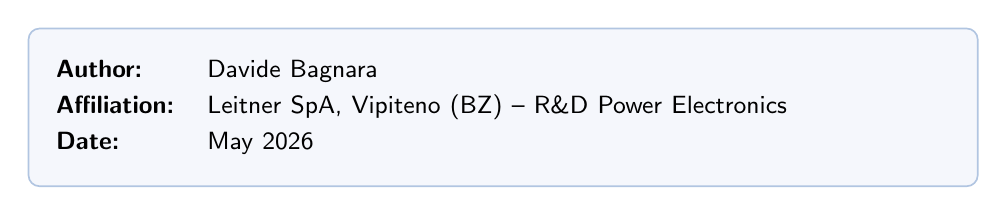
\begin{tikzpicture}
  \node[
      fill      = boxbg,
      draw      = ruleblue!40,
      line width = 0.6pt,
      rounded corners = 4pt,
      inner sep = 10pt,
      text width = \linewidth - 22pt
  ]{%
    \small\sffamily
    \begin{tabular}{@{}ll}
      \textbf{Author:} & \DocAuthor \\[2pt]
      \textbf{Affiliation:} & \DocAffiliation \\[2pt]
      \textbf{Date:} & \DocDate
    \end{tabular}
  };
\end{tikzpicture}

\vspace{18pt}

% ---- Abstract ----
\begin{mdframed}[
    backgroundcolor = abstractbg,
    linecolor       = ruleblue!50,
    linewidth       = 0.8pt,
    leftmargin      = 0pt,
    rightmargin     = 0pt,
    innerleftmargin = 10pt,
    innerrightmargin= 10pt,
    innertopmargin  = 8pt,
    innerbottommargin=8pt,
    roundcorner     = 4pt
]
  \noindent{\small\textbf{Abstract:}\quad\DocAbstract}
\end{mdframed}

\vspace{18pt}

% ---- Metadati tecnici (3 voci) ----
{\color{ruleblue}\hrule height 0.6pt}
\vspace{8pt}

\noindent
\begin{tabularx}{\linewidth}{@{} l X @{}}
    \small\sffamily\textbf{\MetaLabelA:} & \small\sffamily\MetaValueA \\[4pt]
    \small\sffamily\textbf{\MetaLabelB:} & \small\sffamily\MetaValueB \\[4pt]
    \small\sffamily\textbf{\MetaLabelC:} & \small\sffamily\MetaValueC \\
\end{tabularx}

\vspace{8pt}
{\color{ruleblue}\hrule height 0.6pt}

% =============================================================
%   Fine frontespizio — riprendi numerazione per il resto
% =============================================================
\newpage
\pagenumbering{arabic}
\setcounter{page}{1}

% ---- Qui inizia il corpo del documento ----
% \tableofcontents
% \newpage
% \section{Introduction}
% ...

\end{document}
